\documentclass[a4paper]{book}
\usepackage[paper=a4paper]{geometry}% Just for this example
\title{Spevník piesní z regiónu Stredné Považie}
\usepackage{graphics}
\begin{document}
\maketitle
\begin{center}

\chapter*{Stredné Považie}
\section*{Selec}
{%
\parindent 0pt
\noindent
\ifx\preLilyPondExample \undefined
\else
  \expandafter\preLilyPondExample
\fi
\def\lilypondbook{}%

\includegraphics{./61/lily-3c3b53ae-1}%
\ifx\betweenLilyPondSystem \undefined
  \linebreak
\else
  \expandafter\betweenLilyPondSystem{1}%
\fi
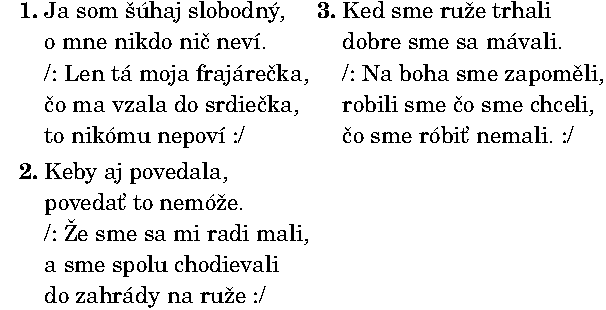
\includegraphics{./61/lily-3c3b53ae-2}%
% eof

\ifx\postLilyPondExample \undefined
\else
  \expandafter\postLilyPondExample
\fi
}
{%
\parindent 0pt
\noindent
\ifx\preLilyPondExample \undefined
\else
  \expandafter\preLilyPondExample
\fi
\def\lilypondbook{}%

\includegraphics{./9d/lily-24819cf1-1}%
\ifx\betweenLilyPondSystem \undefined
  \linebreak
\else
  \expandafter\betweenLilyPondSystem{1}%
\fi

\includegraphics{./9d/lily-24819cf1-2}%
% eof

\ifx\postLilyPondExample \undefined
\else
  \expandafter\postLilyPondExample
\fi
}
{%
\parindent 0pt
\noindent
\ifx\preLilyPondExample \undefined
\else
  \expandafter\preLilyPondExample
\fi
\def\lilypondbook{}%

\includegraphics{./62/lily-acc34dcb-1}%
\ifx\betweenLilyPondSystem \undefined
  \linebreak
\else
  \expandafter\betweenLilyPondSystem{1}%
\fi
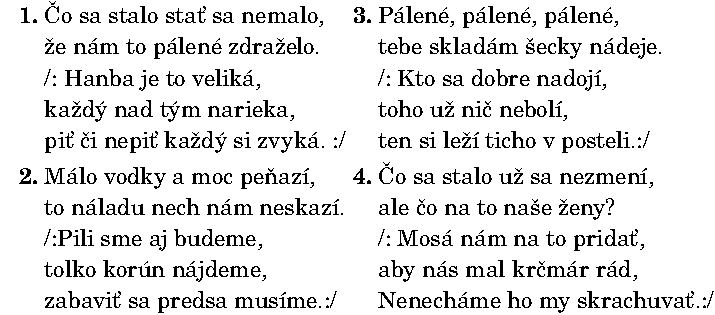
\includegraphics{./62/lily-acc34dcb-2}%
% eof

\ifx\postLilyPondExample \undefined
\else
  \expandafter\postLilyPondExample
\fi
}
{%
\parindent 0pt
\noindent
\ifx\preLilyPondExample \undefined
\else
  \expandafter\preLilyPondExample
\fi
\def\lilypondbook{}%
\includegraphics{./46/lily-fc7a5563-1}%
\ifx\betweenLilyPondSystem \undefined
  \linebreak
\else
  \expandafter\betweenLilyPondSystem{1}%
\fi

\includegraphics{./46/lily-fc7a5563-2}%
% eof

\ifx\postLilyPondExample \undefined
\else
  \expandafter\postLilyPondExample
\fi
}
{%
\parindent 0pt
\noindent
\ifx\preLilyPondExample \undefined
\else
  \expandafter\preLilyPondExample
\fi
\def\lilypondbook{}%

\includegraphics{./3b/lily-a6ce30eb-1}%
\ifx\betweenLilyPondSystem \undefined
  \linebreak
\else
  \expandafter\betweenLilyPondSystem{1}%
\fi
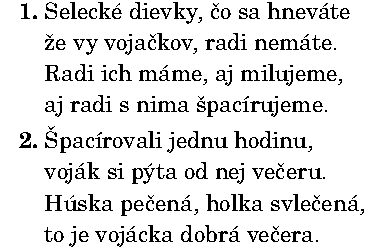
\includegraphics{./3b/lily-a6ce30eb-2}%
% eof

\ifx\postLilyPondExample \undefined
\else
  \expandafter\postLilyPondExample
\fi
}


\end{center}
\end{document}